\documentclass[12pt]{article}

\usepackage[spanish]{babel}
\usepackage[utf8]{inputenc}
\usepackage{graphicx}
\usepackage{geometry}
\usepackage{xcolor}
\usepackage{fancyhdr}
\usepackage{lastpage}
\usepackage{pdfpages}
\usepackage{listings}

\geometry{top=25mm,left=15mm,right=15mm,a4paper}

\pagestyle{fancy}
\fancyhf{}
\lhead{Sistemas Operativos}
\cfoot{Página \thepage\ de \pageref{LastPage}}

\graphicspath{./}

\begin{document}
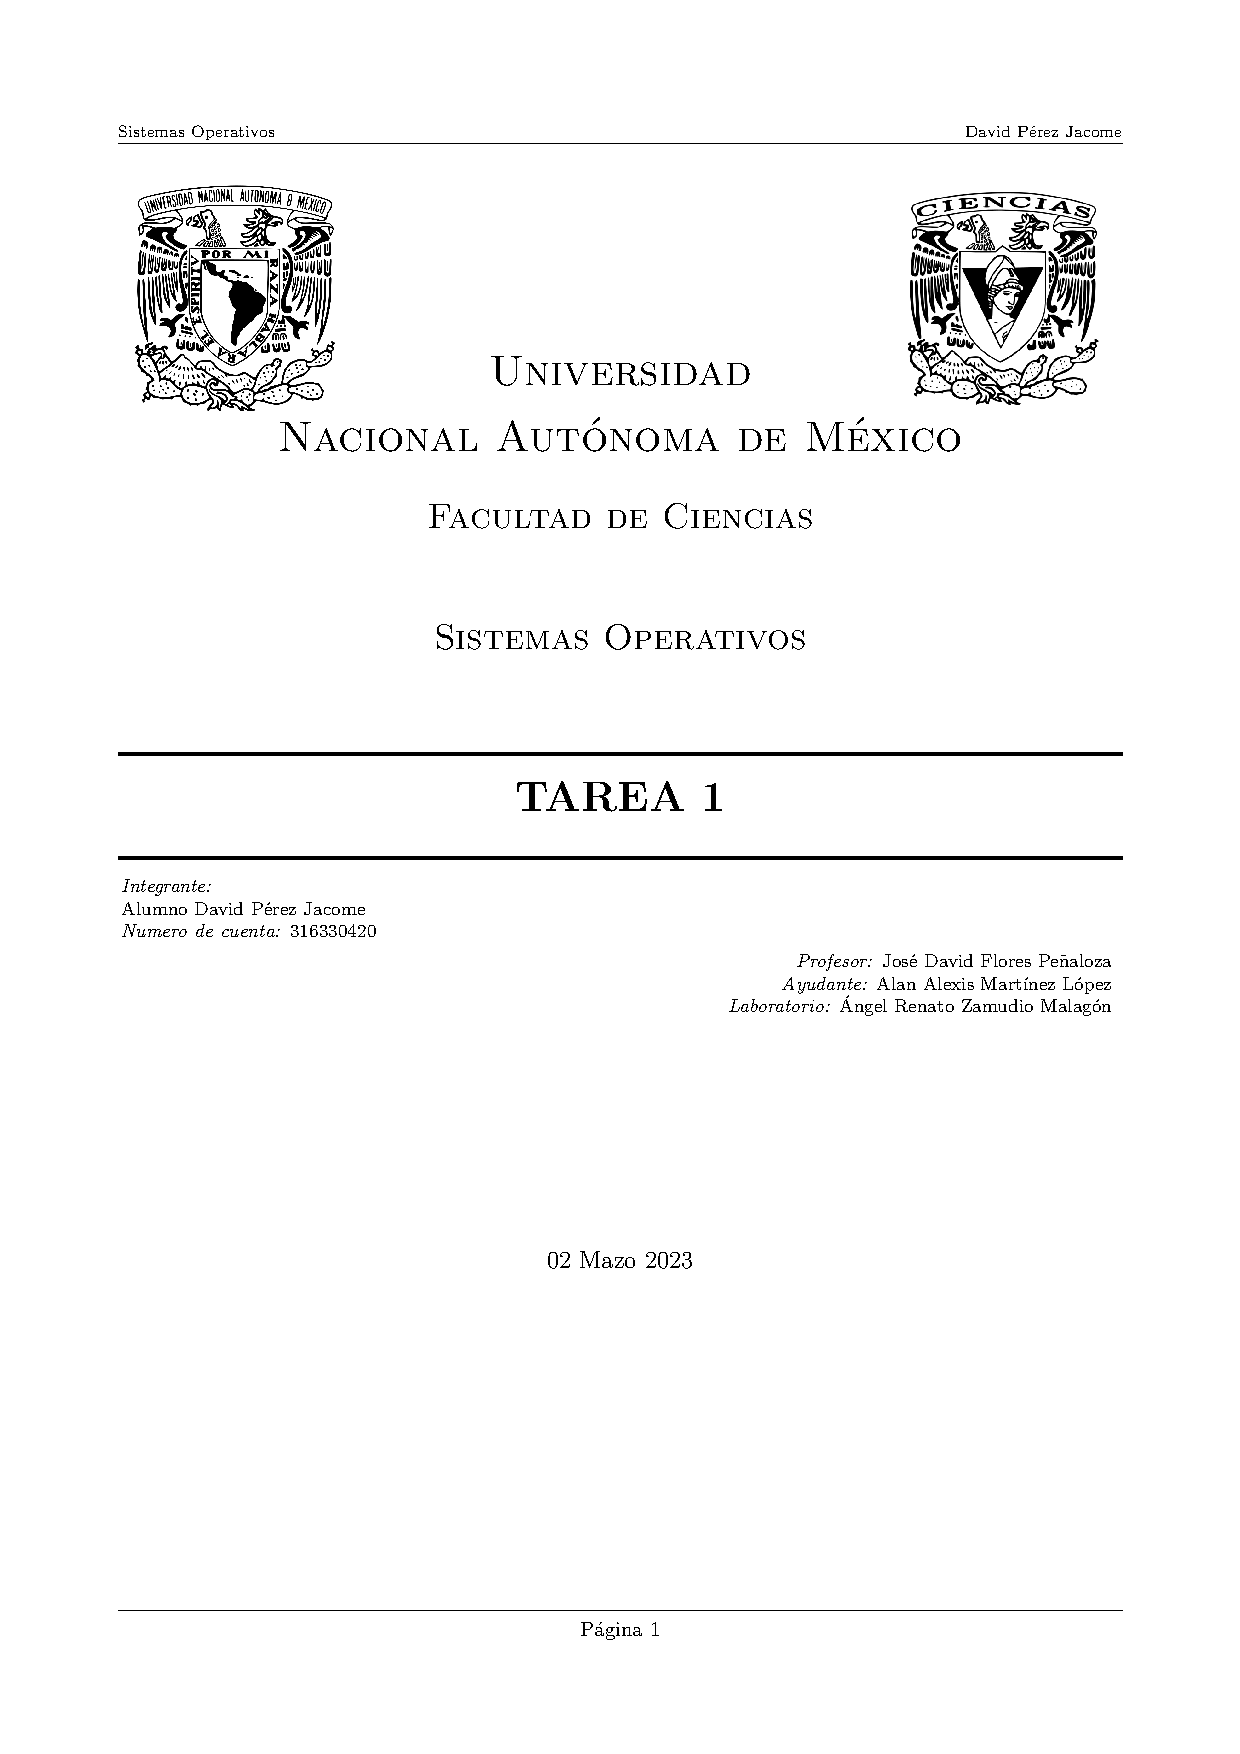
\includepdf{Portada.pdf}
{\color{blue} \section*{Tarea 1.}}

{\color{blue} \subsection*{Instrucciones.}}
\vspace{0.5em} 

Lee con atención las preguntas y contesta lo correspondiente. La tarea se entregará por vía classroom
en un archivo pdf que debe tener el nombre completo y número de tarea, ya sea en una portada o en el encabezado.
\textbf{La tarea se entregará de manera individual.}\\

{\color{blue} \subsection*{Ejercicios}}
\vspace{0.5em}

\begin{enumerate}
    \item Describe brevemente y con tus palabras. ¿Qué es un Sistema Opertivo?
    \vspace{2mm}

    \textbf{Un sistema operativo es un administrador y gestor de recursos requeridos por los procesos.}

    \item ¿Cuáles son las principales tareas de un sistema operativo?
    \vspace{2mm}

    \textbf{\begin{enumerate}
        \item Cargar programas y ejecutarlos.
        \item Dar memoria a los procesos.
        \item Dar tiempo de procesador.
        \item E/S de alto nivel.
        \item Ofrece recursos graficos.
        \item Administración de la energia.
    \end{enumerate}}
    \item ¿Cúales son los pasos a seguir que siempre debe hacer un \textbf{CPU} (microprocesador)? Explicalas brevemente.
    \vspace{2mm}

    \textbf{El ciclo de Instrucciones es:
    \begin{enumerate}
        \item FETCH: Obtener o buscar las instruciones.
        \item DECODE: De que trata (decodificación).
        \item EXECUTE: Ejecución de la instrucción.
        \item WRITE: Se escribe en el caso de sincronia para el proceso.
    \end{enumerate}}
    \item Describe las caracteristicas principales de la memoria primaria. Y menciona un ejemplo.
    \vspace{2mm}

    \textbf{Las caracteristicas de la memoria primaria son:
    \begin{enumerate}
        \item Facil acceso del procesador hacia los datos de la memoria.
        \item Es volatil.
        \item Ayuda a la multitarea.
        \item Acceso aleatorio.
        \item Es mucho más veloz.
        \item Tiene poca capacidad en comparación a otros tipo de memoria.
    \end{enumerate}
    Un ejemplo de este tipo de memoria es la memoria RAM, es la memoria principal de un dispositivo, donde se almacenan de forma temporal 
    los datos de los programas que estás utilizando en este momento.}

    \textbf{}
    \item Describe las caracteristicas principales de la memoria secundaria. Y menciona un ejemplo.
    \vspace{2mm}

    \textbf{Las caracteristicas de la memoria secundaria son:
    \begin{enumerate}
        \item Tiene mayor capacidad de almacenamiento.
        \item No pierde la información.
        \item Alta velocidad en transferencia de información.
        \item Es considerado un dispositivo de almacenamiento externo.
        \item EL procesador no puede acceder directamente a ella, necesita de la caché.
    \end{enumerate}
    Un ejemplo de este tipo de memoria es la memoria Flash/SSD, la cual es unidad de estado sólido proporciona memoria flash continua. Es muy rápido en comparación con los discos duros. A menudo se encuentra en teléfonos 
    móviles y se acepta rápidamente en PC / Laptop / Mac.}

    \item ¿Por qué se cambio la arquitectura de un sistema de computo de un solo procesador a multiprocesadores?
    \vspace{2mm}

    \textbf{Por mejora de rendimineto, ya que facilita la ejecución de varias tareas de manera simultanea, mejora en el sistema al agregar una mayor cantidad de procesadores (escalabilidad),
    en caso de la falla de algún procesador el sistema puede seguir funcionando con el resto (confiablidad) y una facil adaptación a cargas de trabajo (flexibilidad).}
    \item ¿Por qué los sistemas de computo son orientados a interrupciones?
    \vspace{2mm}

    \textbf{Porque es necesario para el proceso de multitareas, el proceso de interrupciones lo que hace es simplemente
    interrumpir una tarea para realizar otra con mayor importancia, esto para que las tareas no se adueñen del procesador.}
    \item ¿Qué es una interrupción de software y para qué se utilizan?
    \vspace{2mm}

    \textbf{Es una llamada "Señal o Signals" y son mensajes enviados por el sistema operativo al proceso en ejecución. También puede verse como una forma de atender eventos, es decir,  permiten interrumpir 
    la ejecución de un proceso para atender la ocurrencia de un evento o bien pueden ser generadas sincrónicamente mediante un error en la aplicación, es el caso de SIGFPE y SIGSEGV. }
    \item ¿Qué es un controlador de dispositivo?
    \vspace{2mm}

    \textbf{Un controlador de dispositivo o driver es un programa de software que tiene subrutinas especificas del dispositivo en cuestión (impresora, mouse, teclado, etc) que toma las
    instruciones d ealto nivel y las comunica a bajo nivel para que las ejecute el controlador y este informe al CPU} 
\end{enumerate}

\end{document}